\documentclass[11pt, oneside]{article}   	% use "amsart" instead of "article" for AMSLaTeX format
%\usepackage{geometry}                		% See geometry.pdf to learn the layout options. There are lots.
\usepackage{listings}
%\geometry{letterpaper}                   		% ... or a4paper or a5paper or ... 
%\geometry{landscape}                		% Activate for for rotated page geometry
\usepackage[parfill]{parskip}    			% Activate to begin paragraphs with an empty line rather than an indent
\usepackage{graphicx}				% Use pdf, png, jpg, or eps§ with pdflatex; use eps in DVI mode
								% TeX will automatically convert eps --> pdf in pdflatex
\usepackage{float}
\usepackage{subcaption}		
\usepackage{amssymb}
\usepackage{listings}
\usepackage[dvipsnames]{xcolor}
\usepackage{fancyvrb}
\usepackage{hyperref}
\graphicspath{ {images/} } 


\newcommand{\verbatiminput}[1]{%
  \VerbatimInput[
    frame=lines,
    framesep=2em,
    label=\fbox{\color{Black}{#1}},
    labelposition=topline,
  ]{#1}%
}

\title{Progetto SISTEMI OPERATIVI 2019-2020}
\author{Simone Cappabianca - Mat: 5423306 \\  simone.cappabianca@stud.unifi.it}
\date{Dicembre 31, 2020}							% Activate to display a given date or no date

\setlength{\parindent}{4em}
\setlength{\parskip}{1em}


\begin{document}

\maketitle
\newpage

\tableofcontents
\newpage

\section{Istruzioni per la compilazione e esecusione}
Per la compilazione del progetto sono necessarie le seguneti librerie aggiuntive:
\begin{itemize}
	\item \textit{libbsd-dev};
	\item \textit{uuid-runtime};
	\item \textit{libuuid-devel}.
\end{itemize} 

Per la prima installazione prima \'e necessario procedere prima alla compilazione del codice sorgente eseguendo il comando \textit{make}. Se la compilazione ha avuto esito positivo si pu\'o procedere all'installazione eseguendo il comando \textit{make install}. Se l'installazione ha avuto esito positivo si pu\'o eseguire il comando \textit{make clean}. Per disinstallare il progetto \'e sufficiente esecuire il comando \textit{make uninstall}. \par

\section{Sistema obiettivo}
Il progetto \'e stato sviluppato sulla distribuzione linux \textbf{Ubuntu 16.04.6 LTS}.

\section{Elementi Facoltativi}
\begin{tabular}{|p{0.4\textwidth}|p{0.2\textwidth}|p{0.4\textwidth}|}
	\hline 
	\textbf{Elemento Facoltativo} & \textbf{Realizzato (SI/NO)} & \textbf{Metodo o file principale}\\
	\hline
	Utilizzo Makefile per la compilazione & \textbf{SI} & \textit{Makefile}\\
	\hline
	Organizzazione in folder, e creazione dei folder al momento della compilazione & \textbf{SI} & \textit{Makefile} \\
	\hline
	Riavvio di PFC1, PFC2, PFC3 alla ricezione di EMERGENZA &  & \\
	\hline
	Utilizzo macro nel Generatore Fallimenti per indicare le probabilità & \textbf{SI} & \textit{common.h} \\
	\hline
	PFC Disconnect Switch sblocca il processo se bloccato, e lo riavvia altrimenti & \textbf{SI} (solo nel caso in cui processo si status \textit{Stopped}) & \textit{disconnect\_switch.c} e \textit{gpgll.c}\\
	\hline
	(continua da sopra) In entrambi i casi, il processo in questione deve riprendere a leggere dal punto giusto del file G18.txt. & & \\
	\hline
\end{tabular}


\section{Progettazione e implementazione}
Tutte le macro di carattere generale che permettono di configurare il progetto sono state definite all'interno del file \texttt{common.h} tra queste ci sono anche quelle che indicano le probabilit\'a con cui vengono lanciati i segnali \textbf{SIGINT}, \textbf{SIGSTOP}, \textbf{SIGCONT} e \textbf{SIGUSR1} e sono rispettivamente \textit{FAILURE\_SIGINT }, \textit{FAILURE\_SIGSTOP}, \textit{FAILURE\_SIGCONT} e \textit{FAILURE\_SIGUSR1}. Se vogliamo  che la probabilit\'a che un determinato segnate sia di $10^-4$ allora la macro corrispondente dovr\'a essere valorizzata con valore 10000.\par  

Il progetto \'e composto da un processo principale \textit{Project} che crea 5 nuovi processi: uno per il \textit{Disconnect Switch}, uno per il \textit{WES}, uno per il \textit{Tranducers}, uno per il \textit{PFCS} e uno per il \textit{Failure Generator}. A sua volta il precesso per il \textit{PFCS} crea a sua volta 4 nuovi processi: uno per il \textit{PFC 1}, uno per il \textit{PFC 2}, uno per il \textit{PFC 3} e uno specifico che si occupa di leggere la coordinata e di sovrascrivela in uno spefico file temporaneo (\textit{reading.tmp}), i tre processi pfc leggeranno la nuova coordinata da questo file. Il processo di lettura legger\'a una coordinata al secondo mentre i tre processi pfc leggeranno il file tempoprane con una frequenza maggiore, per far capire ai pfc che si tratta di una nuova coordinata il processo lettore aggiunge un \textbf{UUID} come prefisso di ogni coordinata scritta nel file temporaneo.\par

Se esaminiamo la procedura di lettura nello spefico si pu\'o notare che \'e composta dalla seguenti fasi:
\begin{itemize}
	\item Nella prima fase viene letto il file \texttt{G18.txt} per creare il file \texttt{GPGLL.txt} che contiene solamente le righe del file \texttt{G18.txt} che iniziano con il prefisso \textit{GPGLL}.
	\item Nella seconda fase viene letto il file creato nella prima fase \texttt{GPGLL.txt} ed il valora letto viene copiato nel file temporaneo \texttt{reading.tmp} che viene utilizzato dai processi PFC.
\end{itemize}
Il nuovo file \texttt{GPGLL.txt} viene gestito come una \textbf{QUEUE} una struttura dati di tipo \textbf{FIFO} (\textit{First-In-First-Out}) questo garantisce che una coordinata venga letta una ed una solo volta. La scelta di far consumare ai vari processi \textit{PFC} un file temporaneo, che contiene una solo coordinata, invece che direttamente il file \texttt{G18.txt} garantisce che nel caso in cui un processo \textit{PFC} venga momentaneamente fermato e successivamente riavviato riprenda a leggere dalla giusta coordinata e sia sincronizzato con gli altri processi.\par

La comunicazione tra il \textit{WES} e il \textit{Disconnect Switch} \'e stata realizzata attraverso l'utilizzo di una \texttt{pipe}.\par 

Sia il processo di \textit{Failure Generator} che il processo di \textit{DisconnectSwitch} hanno la necessit\'a di inviare dei segnali a degli specifici processi durante la loro esecuzione. Per poter inviare questi segnali entrambi \textit{Failure Generator} che \textit{Disconnect Switch} devono conoscere i pid dei processi, per rispondere a questa esigenza tutti i pid dei procesi che servono sia al \textit{FailureGenerator} che al \textit{Disconnect Switch} vengono salvati in specifici file temporanei, per l'esattezza per ogni \textbf{pid} si ha uno specifoco file temporaneo. Il percorso di questi file temporanei \'e indicato all'interno del file \texttt{common.h} \par

\newpage
\begin{figure}[h!]
	\centering
	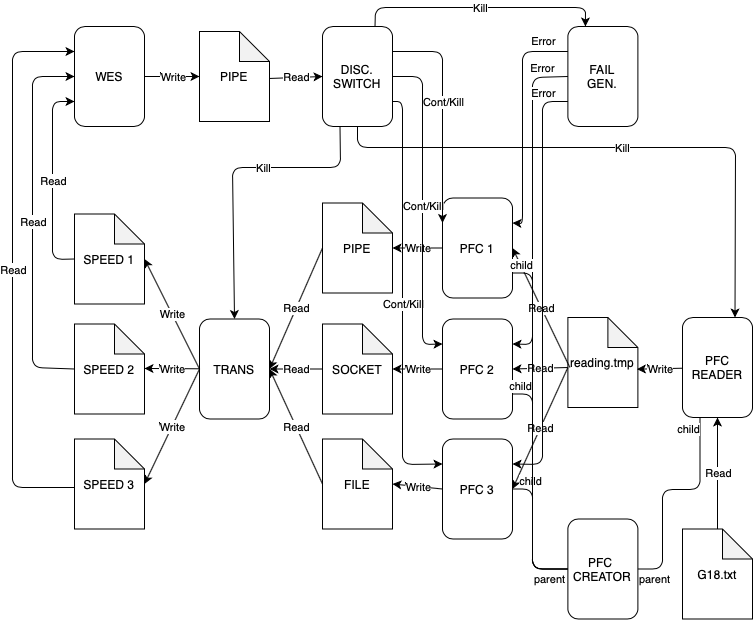
\includegraphics[scale=0.5]{schema.png}
\end{figure}
    
\section{Esecuzione}

In \textit{Appendice} sono riportati i file di log \textbf{STATUS\_20200131.log} e \textbf{FAILURE\_20201231.log} che mostrano un esempio di esecuzione del programma. Da questo esempio di esecuzione \'e interessante analizzare le seguenti situazioni:
\begin{itemize}
	\item gli errori \textit{[20201231-11:27:44:191]:07C5D725-18AA-4C49-AC74-A723F9E2FF1D}, \textit{[20201231-11:27:46:293]:3BBAB173-07F1-4EF4-AB21-F5651CF14773}, \textit{[20201231-11:27:47:344]:2E69E71B-D44F-4539-B564-77CC2687EEA0}  mostra errori di sincronizzazione di lettura delle velocit\'a;
	\item l'errore \textit{[20201231-11:27:53:650]:B5E83716-32B7-4C30-A967-A0CA5D662934} un errore di tipo \textbf{SIGUSR1} come comferma anche la riga di log \textit{[20201231-11:27:53:042]:FAILURE - Type: SIGUSR1 - Process: PFC 02 - PID: 17734} del file \textbf{FAILURE\_20201231.log};
	\item gli errori \textit{[20201231-11:29:00:909]:6021B4D7-41F9-4740-B584-15407E77E06E} al  \textit{[20201231-11:29:19:826]:9EBF0E68-9E13-4A50-A554-DEE6BB9F2138} sono una conseguenza del signale \textbf{SIGSTOP} e \textbf{SIGCONT} come confermato le righe di log \textit{[20201231-11:29:00:058]:FAILURE - Type: SIGSTOP - Process: PFC 01 - PID: 17733} e \textit{[20201231-11:29:20:063]:FAILURE - Type: SIGCONT - Process: PFC 01 - PID: 17733} del file \textbf{FAILURE\_20201231.log};
	\item l'errore \textit{[20201231-11:29:27:183]:8C130A56-CBC5-4307-AB4E-39AA6EC8E9C6}  di \textbf{EMERGENCY} \'e stato generato dalla concomitanza di una mancata sincronizzazione di lettura delle velocit\'a e di un errore di tipo \textbf{SIGUSR1} come si conferma la riga di log \textit{[20201231-11:29:27:065]:FAILURE - Type: SIGUSR1 - Process: PFC 03 - PID: 17735} del file \textbf{FAILURE\_20201231.log}.
\end{itemize}

\newpage

\section{Appendice}
\begin{Verbatim}[frame=topline,
			framesep=4mm,
			label=\fbox{\Large{STATUS\_20201231.log}}]
[20201231-11:27:41:039]:05457FC1-AF49-4134-B0B6-B8497A09D2CB - STATUS: OK        
- (1067.860822, 1067.860822, 1067.860822)
[20201231-11:27:42:090]:90EA9F11-9B05-4776-8866-D049F5A8550F - STATUS: OK        
- (205.380501, 205.380501, 205.380501)
[20201231-11:27:43:140]:AC370A44-2138-4CA1-B45A-1D58F8172733 - STATUS: OK        
- (309.985845, 309.985845, 309.985845)
[20201231-11:27:44:191]:07C5D725-18AA-4C49-AC74-A723F9E2FF1D - STATUS: ERROR     
- (32.708111, 84.541128, 32.708111)
[20201231-11:27:45:242]:EAAC98DA-E476-47D1-A170-B0225CCA94EF - STATUS: OK        
- (84.541128, 84.541128, 84.541128)
[20201231-11:27:46:293]:3BBAB173-07F1-4EF4-AB21-F5651CF14773 - STATUS: ERROR     
- (89.495411, 36.012617, 36.012617)
[20201231-11:27:47:344]:2E69E71B-D44F-4539-B564-77CC2687EEA0 - STATUS: ERROR     
- (36.012617, 66.869123, 66.869123)
[20201231-11:27:48:395]:3A801374-3E92-4382-8276-4ED352CDAEF7 - STATUS: ERROR     
- (66.869123, 44.267293, 44.267293)
[20201231-11:27:49:446]:6D1EE4E9-8776-41F2-8A87-FB6D3E75C11E - STATUS: OK        
- (23.868686, 23.868686, 23.868686)
[20201231-11:27:50:497]:5A598059-A6BE-4D0E-BFF0-38D284524DD1 - STATUS: OK        
- (28.624932, 28.624932, 28.624932)
[20201231-11:27:51:547]:C93DCA01-9940-406E-A4AE-8B78DD035AFB - STATUS: OK        
- (16.835951, 16.835951, 16.835951)
[20201231-11:27:52:599]:BD93F73F-6308-4EEC-A738-6FCE0279C6ED - STATUS: OK        
- (11.934329, 11.934329, 11.934329)
[20201231-11:27:53:650]:B5E83716-32B7-4C30-A967-A0CA5D662934 - STATUS: ERROR     
- (13.376770, 52.000000, 13.376770)
[20201231-11:27:54:701]:249C7D47-86E3-4519-AF0A-E1F88073F5D4 - STATUS: OK        
- (4.001402, 4.001402, 4.001402)
[20201231-11:27:55:751]:BB0E733B-2255-4062-8BBA-79820C2B8472 - STATUS: ERROR     
- (32.146961, 128.000000, 32.146961)
[20201231-11:27:56:803]:8F8F7442-7721-4069-A27E-EB6C883A2B7C - STATUS: OK        
- (34.803752, 34.803752, 34.803752)
[20201231-11:27:57:854]:F664C5C1-8DC6-4606-B9CA-7E76998535D6 - STATUS: OK        
- (45.031900, 45.031900, 45.031900)
[20201231-11:27:58:905]:4266C178-A825-4A1F-BB27-D0F023A6B129 - STATUS: ERROR     
- (4.971961, 16.000000, 4.971961)
[20201231-11:27:59:956]:23E61609-30B6-4CFE-B4C3-15B849AC89EF - STATUS: OK        
- (4.001402, 4.001402, 4.001402)
[20201231-11:28:01:007]:68B4BEEB-90F7-4D58-9ED6-478A369CEE42 - STATUS: OK        
- (4.001402, 4.001402, 4.001402)
[20201231-11:28:02:057]:4A56090B-FC42-49E5-9D7C-91E35C50D22B - STATUS: OK        
- (16.835911, 16.835911, 16.835911)
[20201231-11:28:03:108]:95C5283A-CADD-4D94-985F-A3731DCDEFCF - STATUS: OK        
- (23.868608, 23.868608, 23.868608)
[20201231-11:28:04:159]:4DE7E0AF-24DF-4711-9B39-2BD8B11001E7 - STATUS: OK        
- (28.523124, 28.523124, 28.523124)
[20201231-11:28:05:210]:85CDCB06-AC84-465B-8E33-4BF482493865 - STATUS: OK        
- (24.189110, 24.189110, 24.189110)
[20201231-11:28:06:261]:C8C7E79E-891D-4467-927F-5F13077E906B - STATUS: OK        
- (24.189110, 24.189110, 24.189110)
[20201231-11:28:07:311]:ED62CBAE-DAF1-472D-9060-1B75BC417CBA - STATUS: OK        
- (23.868661, 23.868661, 23.868661)
[20201231-11:28:08:362]:41FE1248-CDB1-4723-A8D9-44A752AB6E6B - STATUS: OK        
- (17.059208, 17.059208, 17.059208)
[20201231-11:28:09:413]:CCD4476B-4066-4E2C-AFC1-0FE9C62C2BD9 - STATUS: OK        
- (20.859472, 20.859472, 20.859472)
[20201231-11:28:10:464]:0AAE03B8-5125-4783-9392-85483ED5E58D - STATUS: OK        
- (14.915919, 14.915919, 14.915919)
[20201231-11:28:11:515]:735BF502-581D-4A0B-AD3E-FB31E5154BB7 - STATUS: OK        
- (13.376778, 13.376778, 13.376778)
[20201231-11:28:12:566]:2D853B45-7594-4C7A-87CC-4D5119A0B990 - STATUS: OK        
- (8.529606, 8.529606, 8.529606)
[20201231-11:28:13:617]:A1C12660-321D-4BDA-84FB-E3AA3F924768 - STATUS: OK        
- (0.000000, 0.000000, 0.000000)
[20201231-11:28:14:668]:A1643ECC-8860-4BDE-BDAF-45874121BE92 - STATUS: OK        
- (12.361645, 12.361645, 12.361645)
[20201231-11:28:15:719]:745C7313-17B0-40EE-ADAF-1962A0F86011 - STATUS: OK        
- (13.376781, 13.376781, 13.376781)
[20201231-11:28:16:770]:41D62C8A-7CAE-49A1-A908-4CBACF3BC154 - STATUS: OK        
- (9.715721, 9.715721, 9.715721)
[20201231-11:28:17:821]:460EDA3C-2B3F-4EF4-8B5B-152CA93D65B9 - STATUS: OK        
- (8.853476, 8.853476, 8.853476)
[20201231-11:28:18:872]:EB435DBC-ED96-4D87-B9CD-C3DB7291A661 - STATUS: OK        
- (13.376782, 13.376782, 13.376782)
[20201231-11:28:19:922]:FA2EB703-E5AE-4F82-830E-286B97B7D6B4 - STATUS: OK        
- (21.878399, 21.878399, 21.878399)
[20201231-11:28:20:974]:45C40394-D672-48B2-A258-7817B636D562 - STATUS: OK        
- (11.804619, 11.804619, 11.804619)
[20201231-11:28:22:024]:4B965C26-5563-4B5E-B67E-892E43FC09E2 - STATUS: OK        
- (2.951155, 2.951155, 2.951155)
[20201231-11:28:23:075]:507AA3B5-E17B-41B8-9B04-8C14044BCAA9 - STATUS: ERROR     
- (4.971975, 4.971975, 16.000000)
[20201231-11:28:24:126]:835B6810-ED4B-4856-8C05-3AA1FB860DC0 - STATUS: OK        
- (5.902310, 5.902310, 5.902310)
[20201231-11:28:25:177]:22228A90-C146-4444-AA91-070C747813D5 - STATUS: OK        
- (12.464362, 12.464362, 12.464362)
[20201231-11:28:26:228]:D804C660-9D63-4734-B008-1810AC8F9642 - STATUS: OK        
- (17.706937, 17.706937, 17.706937)
[20201231-11:28:27:279]:4C2A624B-10AD-41C1-86FE-1544ED7C4A42 - STATUS: OK        
- (17.706937, 17.706937, 17.706937)
[20201231-11:28:28:330]:FA6D1A07-476E-4B4A-B989-4518DE9519B3 - STATUS: OK        
- (14.755781, 14.755781, 14.755781)
[20201231-11:28:29:380]:39808D02-ECD9-45A1-9E4E-7352D1BFAB53 - STATUS: OK        
- (4.971976, 4.971976, 4.971976)
[20201231-11:28:30:431]:CCCA4305-C222-44CC-B5FC-AD9A910A0FC4 - STATUS: OK        
- (19.021934, 19.021934, 19.021934)
[20201231-11:28:31:482]:C24F0789-F3D8-4393-9F14-E9C9C2EA2683 - STATUS: ERROR     
- (8.529606, 32.000000, 8.529606)
[20201231-11:28:32:533]:02AF0444-0365-4F19-9FD4-63D1FBD12DA5 - STATUS: OK        
- (21.878395, 21.878395, 21.878395)
[20201231-11:28:33:584]:3D9DDD69-63CB-4FA7-A868-8F56C427CA84 - STATUS: OK        
- (21.878392, 21.878392, 21.878392)
[20201231-11:28:34:635]:EC1567C9-4156-4E59-BA91-8F73C7AA9001 - STATUS: OK        
- (19.021907, 19.021907, 19.021907)
[20201231-11:28:35:686]:67D5093B-4BDC-4765-8653-CC49BAFAB2C9 - STATUS: OK        
- (26.133000, 26.133000, 26.133000)
[20201231-11:28:36:737]:7F66E104-32B7-419C-AC0F-DB013243EF3A - STATUS: OK        
- (9.715687, 9.715687, 9.715687)
[20201231-11:28:37:788]:293B9BCF-D379-4691-BEDF-E499190FFBF9 - STATUS: OK        
- (8.002804, 8.002804, 8.002804)
[20201231-11:28:38:839]:5E58C156-BBBF-4366-9D92-6FE769B5CD66 - STATUS: OK        
- (5.902293, 5.902293, 5.902293)
[20201231-11:28:39:890]:4CD70AB2-249A-4D39-8A31-42333E31BA63 - STATUS: OK        
- (9.943940, 9.943940, 9.943940)
[20201231-11:28:40:941]:3797C64B-3D3E-410D-9DB1-7E063AA1CB29 - STATUS: OK        
- (21.392403, 21.392403, 21.392403)
[20201231-11:28:41:992]:F281CE8A-796F-433C-8459-EF26434FC747 - STATUS: OK        
- (12.464339, 12.464339, 12.464339)
[20201231-11:28:43:043]:E5F5AEAB-DA3A-4842-989B-0277B5A6C412 - STATUS: OK        
- (9.715698, 9.715698, 9.715698)
[20201231-11:28:44:094]:A88CFC13-8945-4ECC-8AED-96990CD89619 - STATUS: OK        
- (2.951150, 2.951150, 2.951150)
[20201231-11:28:45:145]:B64C95C0-2114-45F1-9757-34E92F5E1E7D - STATUS: OK        
- (9.943944, 9.943944, 9.943944)
[20201231-11:28:46:195]:877D696F-A1DA-4437-846A-02BA74F31097 - STATUS: OK        
- (9.943945, 9.943945, 9.943945)
[20201231-11:28:47:246]:8D40AF44-361D-4E79-A154-6D638BAF4C05 - STATUS: OK        
- (21.392429, 21.392429, 21.392429)
[20201231-11:28:48:297]:6CCE0860-51E0-482B-B21C-13CDDC5CF3EE - STATUS: OK        
- (21.392429, 21.392429, 21.392429)
[20201231-11:28:49:348]:3E3100F4-5773-43C9-B50C-80B07EC6DE37 - STATUS: OK        
- (24.928722, 24.928722, 24.928722)
[20201231-11:28:50:399]:E07CE969-A7DA-46F8-858C-888DFA0A2FCA - STATUS: OK        
- (8.002804, 8.002804, 8.002804)
[20201231-11:28:51:450]:33264B21-53D8-4F21-ACC3-28012400DEF5 - STATUS: OK        
- (8.529607, 8.529607, 8.529607)
[20201231-11:28:52:501]:E6D19088-48B1-48BE-B188-8566DD3AD739 - STATUS: OK        
- (15.288706, 15.288706, 15.288706)
[20201231-11:28:53:552]:5527E3E7-4D9D-4444-8FBD-CFC55F9493D7 - STATUS: OK        
- (32.462739, 32.462739, 32.462739)
[20201231-11:28:54:604]:64685600-9DF4-4F69-8012-F08B5B201B33 - STATUS: OK        
- (29.511581, 29.511581, 29.511581)
[20201231-11:28:55:654]:7571C403-2CF7-4331-B7A5-E41C4A9DC992 - STATUS: OK        
- (23.609265, 23.609265, 23.609265)
[20201231-11:28:56:705]:EF082D96-849F-44B7-8D05-6732F1B52BA9 - STATUS: OK        
- (20.658107, 20.658107, 20.658107)
[20201231-11:28:57:756]:7228AB45-E04A-4AF9-B4CE-6E3F7AF818BE - STATUS: OK        
- (14.755790, 14.755790, 14.755790)
[20201231-11:28:58:807]:AEC7B073-BC00-4F6F-83AE-9B6A5EE4E141 - STATUS: OK        
- (9.943954, 9.943954, 9.943954)
[20201231-11:28:59:858]:3EA0D8E4-10D7-4C7A-87FF-A83CEE226B6B - STATUS: OK        
- (8.002804, 8.002804, 8.002804)
[20201231-11:29:00:909]:6021B4D7-41F9-4740-B584-15407E77E06E - STATUS: ERROR     
- (8.002804, 2.951160, 2.951160)
[20201231-11:29:01:960]:DD0DBCC1-56BD-44C0-86CF-AF5F75F9B0D2 - STATUS: ERROR     
- (8.002804, 8.529608, 8.529608)
[20201231-11:29:03:011]:1F7F3A30-5F3C-4395-922C-FA072E4B556C - STATUS: ERROR     
- (8.002804, 11.934358, 11.934358)
[20201231-11:29:04:062]:EFDEC139-C3FA-4B0B-A30E-8828898A5ACA - STATUS: ERROR     
- (8.002804, 16.835980, 16.835980)
[20201231-11:29:05:113]:8AFE7282-CE18-47F0-B3D5-1E383B34E1B3 - STATUS: ERROR     
- (8.002804, 16.835976, 16.835976)
[20201231-11:29:06:164]:1908C075-4BC3-47AE-943B-46B61248DACC - STATUS: ERROR     
- (8.002804, 16.835968, 16.835968)
[20201231-11:29:07:215]:98DC3CEC-FFB7-4F7A-8742-30A6712653D4 - STATUS: ERROR     
- (8.002804, 16.835968, 16.835968)
[20201231-11:29:08:266]:9AAD0B9E-201C-471D-99BB-8713E13587EC - STATUS: ERROR     
- (8.002804, 7.130807, 7.130807)
[20201231-11:29:09:317]:F4BB17E1-D370-40F7-AA1D-0D03DE531859 - STATUS: ERROR     
- (8.002804, 4.971973, 4.971973)
[20201231-11:29:10:368]:AA8FB7C2-5D54-467B-9266-455C1168B46E - STATUS: ERROR     
- (8.002804, 4.001402, 4.001402)
[20201231-11:29:11:419]:A30161A7-51DF-4B8E-9DC4-4E5A2891A899 - STATUS: ERROR     
- (8.002804, 12.004206, 12.004206)
[20201231-11:29:12:469]:DE2FF0C2-35CC-4420-B843-9AF2E5DD9DD1 - STATUS: ERROR     
- (8.002804, 9.943949, 9.943949)
[20201231-11:29:13:521]:CABD5B8A-5059-47A5-B171-0D3045841F5D - STATUS: ERROR     
- (8.002804, 8.529606, 8.529606)
[20201231-11:29:14:572]:AF370229-A27A-4DA9-A2C5-1F08B6B8AEF1 - STATUS: ERROR     
- (8.002804, 8.529607, 8.529607)
[20201231-11:29:15:622]:3135C19E-C02A-46C0-9746-DC41A664E8AD - STATUS: ERROR     
- (8.002804, 8.529607, 8.529607)
[20201231-11:29:16:673]:22550CDB-AFBB-40FF-A626-9147DDAEF159 - STATUS: ERROR     
- (8.002804, 7.130817, 7.130817)
[20201231-11:29:17:725]:4D87253F-160C-46A1-BD20-343B0E342B8A - STATUS: ERROR     
- (8.002804, 8.002804, 32.000000)
[20201231-11:29:18:776]:8A7CEFE3-5B0D-406F-94AE-DB537958D7F5 - STATUS: ERROR     
- (8.002804, 13.376783, 13.376783)
[20201231-11:29:19:826]:9EBF0E68-9E13-4A50-A554-DEE6BB9F2138 - STATUS: ERROR     
- (8.002804, 29.781637, 29.781637)
[20201231-11:29:20:877]:774E124B-1D9F-4241-818B-ED23200B2181 - STATUS: OK        
- (21.392464, 21.392464, 21.392464)
[20201231-11:29:21:928]:517F3ACE-3251-48EF-851F-FCDCE2F2273D - STATUS: OK        
- (11.934365, 11.934365, 11.934365)
[20201231-11:29:22:979]:C7B13FCC-CD6A-4226-80CC-9DCDFC6EFE15 - STATUS: ERROR     
- (13.376786, 52.000000, 13.376786)
[20201231-11:29:24:031]:FFBC93A2-861B-4142-B32B-9AF055182E12 - STATUS: ERROR     
- (56.000000, 14.261655, 14.261655)
[20201231-11:29:25:081]:70E9A3EF-41AB-4A96-A9A6-BDE36B401118 - STATUS: OK        
- (7.130829, 7.130829, 7.130829)
[20201231-11:29:26:132]:A890A34B-2007-431A-9800-FC32C631C870 - STATUS: OK        
- (4.001402, 4.001402, 4.001402)
[20201231-11:29:27:183]:8C130A56-CBC5-4307-AB4E-39AA6EC8E9C6 - STATUS: EMERGENCY 
- (11.934375, 12.004206, 48.000000)
\end{Verbatim}

\newpage

\begin{Verbatim}[frame=topline,
			framesep=4mm,
			label=\fbox{\Large{FAILURE\_20201231.log}}]
[20201231-11:27:39:038]:FAILURE - SIGINT: 10000 - SIGSTOP : 100 - SIGCONT: 10
 - SIGUSR1: 10
[20201231-11:27:40:039]:FAILURE - Type: SIGCONT - Process: PFC 02 - PID: 17734
[20201231-11:27:53:042]:FAILURE - Type: SIGCONT - Process: PFC 02 - PID: 17734
[20201231-11:27:53:042]:FAILURE - Type: SIGUSR1 - Process: PFC 02 - PID: 17734
[20201231-11:27:55:042]:FAILURE - Type: SIGUSR1 - Process: PFC 02 - PID: 17734
[20201231-11:27:58:043]:FAILURE - Type: SIGUSR1 - Process: PFC 02 - PID: 17734
[20201231-11:28:11:046]:FAILURE - Type: SIGCONT - Process: PFC 02 - PID: 17734
[20201231-11:28:22:049]:FAILURE - Type: SIGUSR1 - Process: PFC 03 - PID: 17735
[20201231-11:28:23:049]:FAILURE - Type: SIGCONT - Process: PFC 03 - PID: 17735
[20201231-11:28:27:050]:FAILURE - Type: SIGCONT - Process: PFC 03 - PID: 17735
[20201231-11:28:27:050]:FAILURE - Type: SIGUSR1 - Process: PFC 03 - PID: 17735
[20201231-11:28:31:051]:FAILURE - Type: SIGUSR1 - Process: PFC 02 - PID: 17734
[20201231-11:28:44:054]:FAILURE - Type: SIGCONT - Process: PFC 03 - PID: 17735
[20201231-11:29:00:058]:FAILURE - Type: SIGSTOP - Process: PFC 01 - PID: 17733
[20201231-11:29:05:059]:FAILURE - Type: SIGCONT - Process: PFC 02 - PID: 17734
[20201231-11:29:09:060]:FAILURE - Type: SIGUSR1 - Process: PFC 01 - PID: 17733
[20201231-11:29:15:062]:FAILURE - Type: SIGCONT - Process: PFC 02 - PID: 17734
[20201231-11:29:17:062]:FAILURE - Type: SIGUSR1 - Process: PFC 03 - PID: 17735
[20201231-11:29:20:063]:FAILURE - Type: SIGCONT - Process: PFC 01 - PID: 17733
[20201231-11:29:22:063]:FAILURE - Type: SIGUSR1 - Process: PFC 02 - PID: 17734
[20201231-11:29:23:064]:FAILURE - Type: SIGCONT - Process: PFC 01 - PID: 17733
[20201231-11:29:23:064]:FAILURE - Type: SIGUSR1 - Process: PFC 01 - PID: 17733
[20201231-11:29:26:064]:FAILURE - Type: SIGCONT - Process: PFC 01 - PID: 17733
[20201231-11:29:27:065]:FAILURE - Type: SIGUSR1 - Process: PFC 03 - PID: 17735
\end{Verbatim}
\end{document}